%-------------------------------------------------------------------
\subsection{Evaluation}
\begin{frame}[t]{Evaluation}
	\begin{itemize}
	 \item \textbf{Prototype:} Java Servlet (Spring Framework) version of Question \& Answers System
	 \item \textbf{Data:} Data crawled from Stackoverflow.com	 	 \item \textbf{Database: }Cassandra and Voldemort (Key-Value store, DynamoDB)
	 \item \textbf{PaaS: }OpenShift, AppScale (Google App Engine) 
	 \item \textbf{IaaS: } OpenStack and Amazon Web Services or Google Cloud Platform
	\end{itemize}    
\note{
Este conceito será testado com uma aplicação protótipo Java Spring baseada num sistema de Question and Answers. Serão usados PaaS opensource Openshift e AppScale. Os pedidos serão guardados na Big Table Cassandra enquanto que a aplicação usará o Voldemort, um key-value store da LinkedIn equivalente ao DynamoDB da Amazon.
}
\end{frame}

\begin{frame}[t]{Evaluation}
	\begin{itemize}
	\item \textbf{Record impact:} Delay, throughput, resource usage, maximum load
	\item \textbf{Replay:} Precision, recall, duration and scalability
	\item \textbf{Integrity and Availability:} Corrupted and unavailable data during recovery
	\item \textbf{Concurrency: }Correctness and performance improvement
	\item \textbf{Cost: }Monetary cost in a public cloud provider
	\end{itemize}
	
\note{
Iremos medir qual o impacto do serviço na aplicação, qual a precisão, recall, duração e escalabilidade do processo de replay. Iremos avaliar se a aplicação consegue permanecer integra e disponivel durante o processo, se o processo de replay em parallel é efectivamente vantajoso e qual o custo de usar esta solução num cloud provider.
} 
\end{frame}
%-------------------------------------------------------------------
\section{Conclusion}
\subsection{Schedule}
\begin{frame}[c]{Schedule}
\vskip-5mm
\makebox[\linewidth][c]{
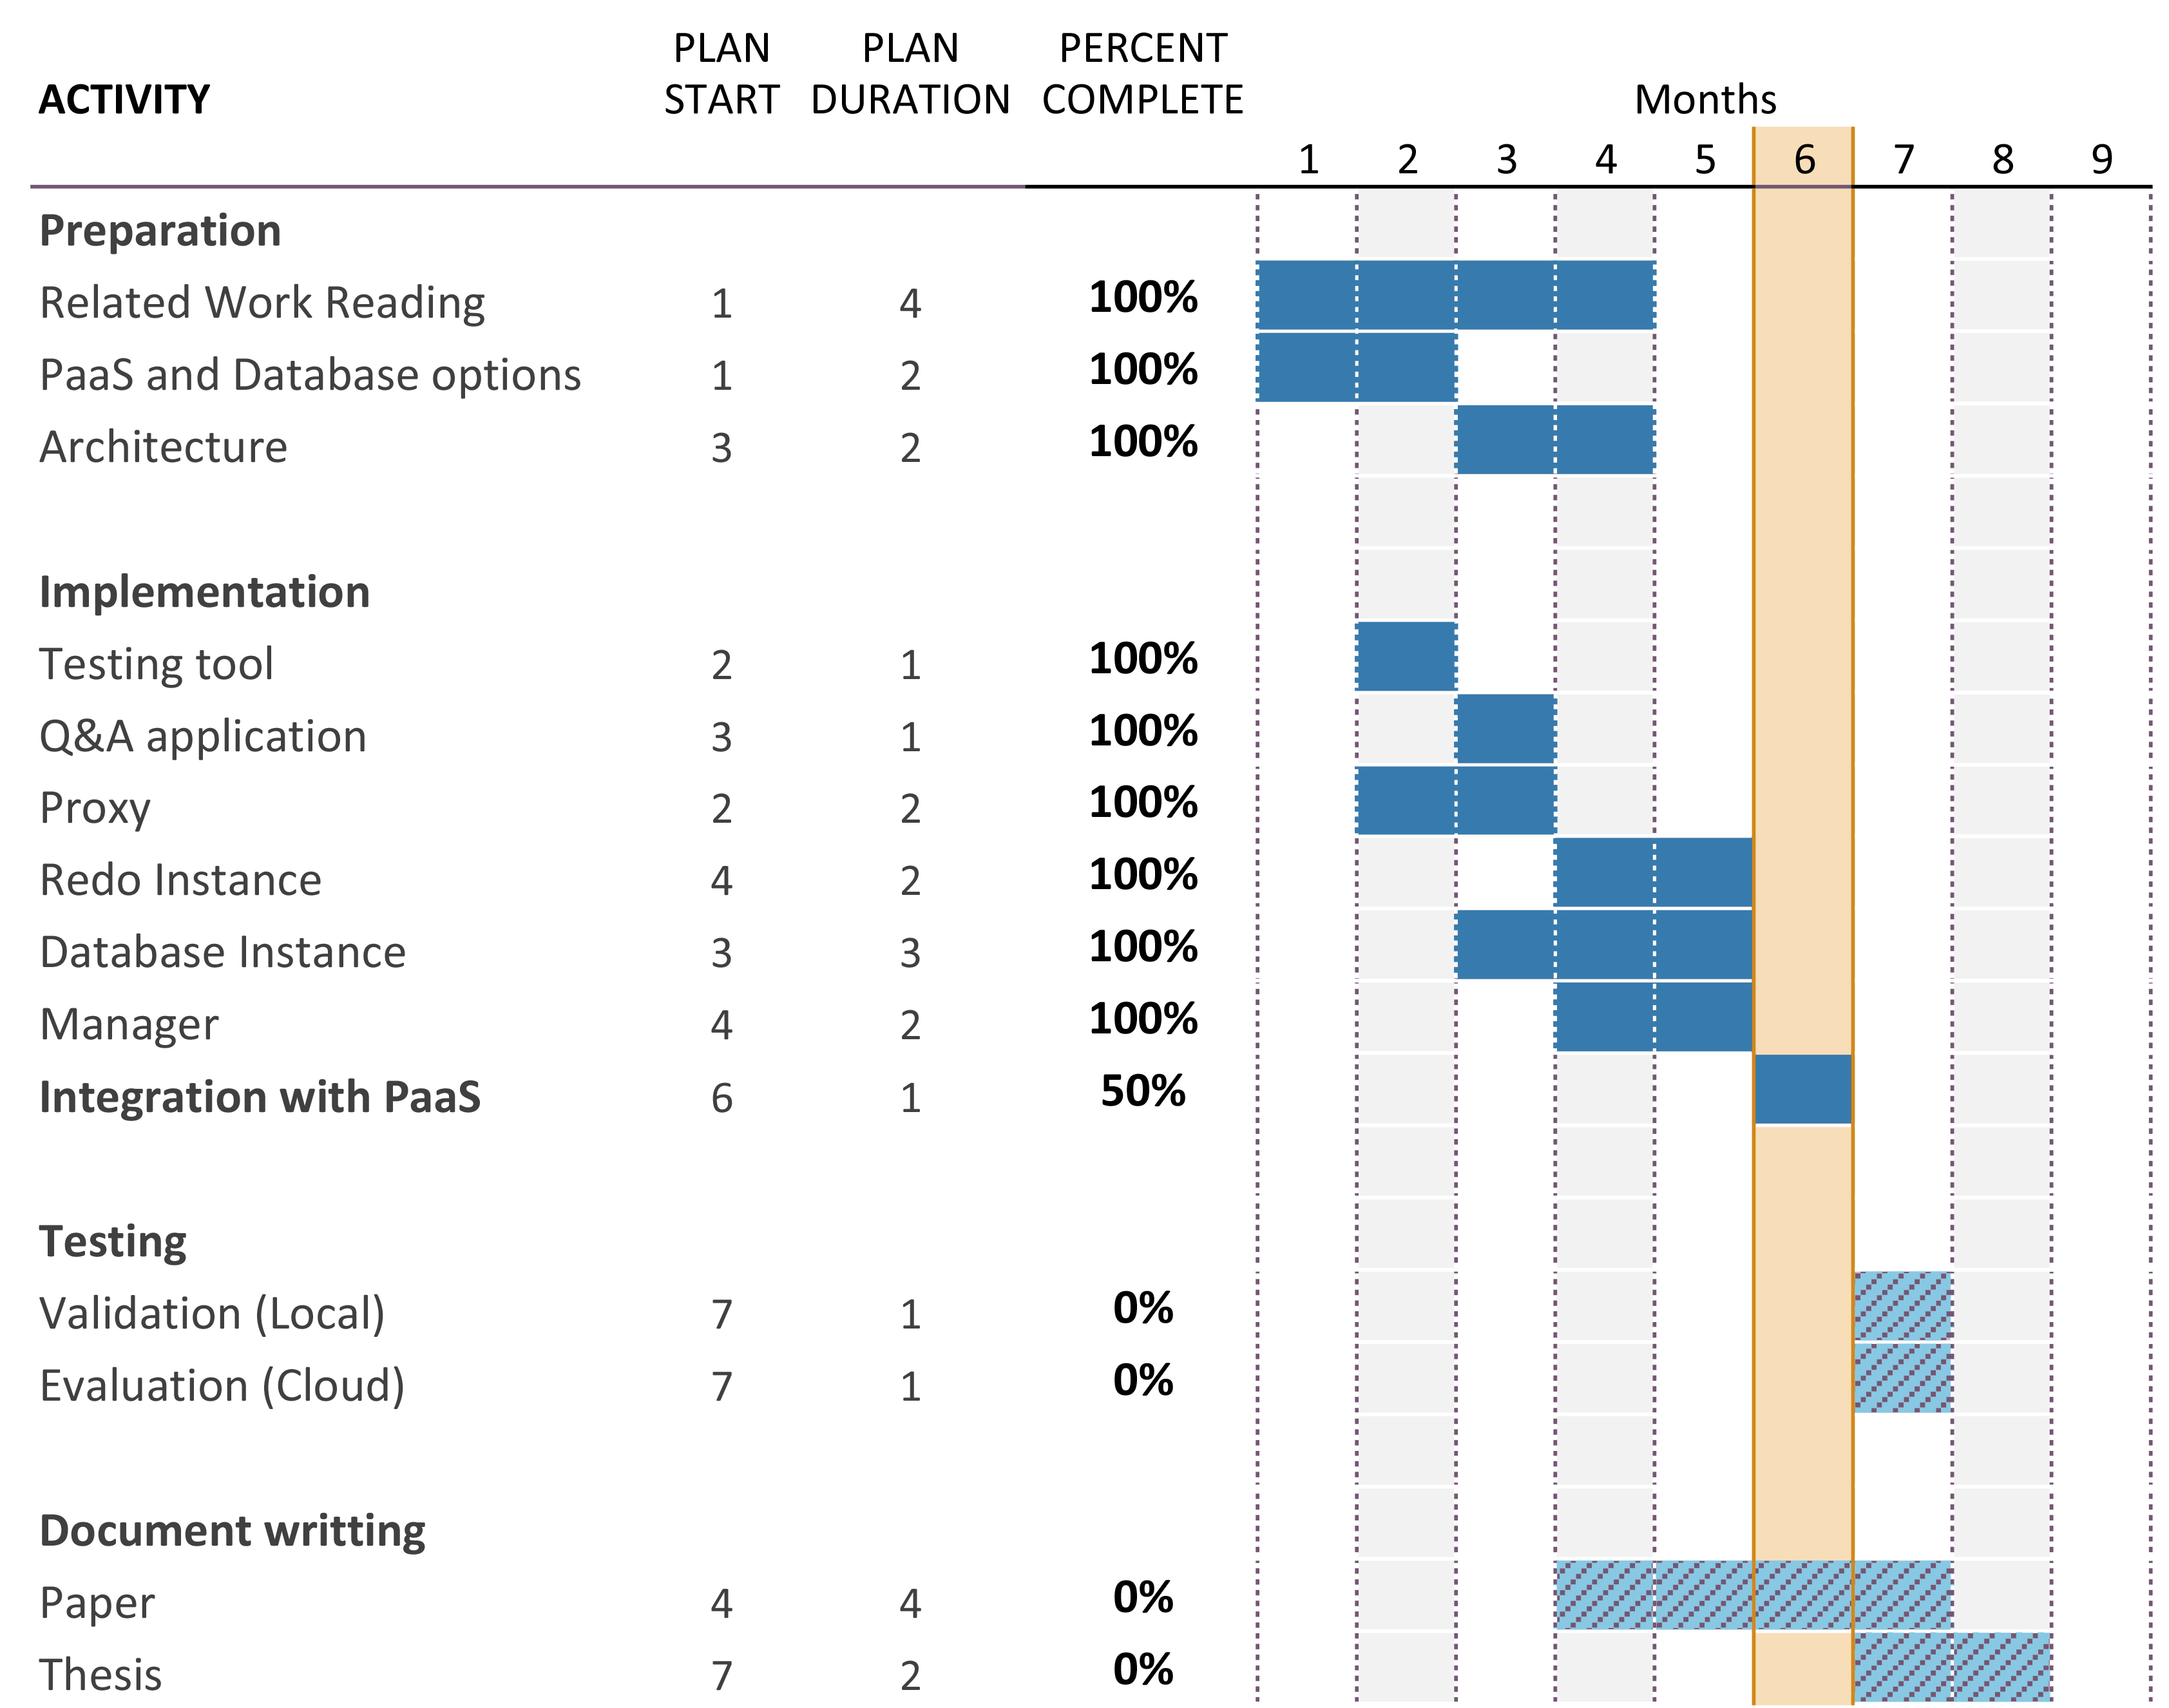
\includegraphics[width=90mm]{img/gantt}
}

\note{
Na fase de preparação comecei por ler e analisar o trabalho relacionado, as opções e arquitectura para PaaS e base de dadoss e fiz uns pequenos testes de conceito usando Python.
} 
\end{frame}



%-------------------------------------------------------------------

\subsection{Conclusion}

\begin{frame}[c]{Conclusion}
    \vskip-0.5cm
	\textbf{Shuttle is the first:}
	\begin{itemize}
	  \setlength{\wideitemsep}{0.3cm}
	  \item  Intrusion recovery service for PaaS using replay
	  \item  To NoSQL databases and snapshoting
	  \item  To concern the parallel replay
	\end{itemize}
	\vskip0.5cm
	\textbf{Amongst the first:}
	\begin{itemize}
	  \setlength{\wideitemsep}{0.3cm}
	  \item  To incorporate the instance renewing
	  \item  To recover without application downtime
	\end{itemize}
	
\note{
Como proposto, o sistema apresentado guarda os pedidos dos utilizadores e as suas dependências para remover os ataques a aplicações deployed em Paas. Mais, conseguimos suportar actualizações de software ou migrar a aplicação para containers limpos.
Pelo que investigámos, este é o primeiro sistema de recuperação para PaaS e o primeiro projecto que aborda o paralelismo do replay e o seu uso em bases de dados não SQL.
Acredito portanto que este sistema apresenta um grande potencial para a comunidade.
} 
\end{frame}
